\chapter{Arquitetura do sistema}\label{cap:arquitetura}

Para conseguirmos estabelecer a comunicação entre o computador e o SoC precisaremos:

\begin{enumerate}
	\item Efetuar programação de \textit{sockets} e bibliotecas específicas para trabalho em redes; 
	
	\item Desenvolver um pacote ROS para disponibilizar os dados recebidos dos outros pacotes ROS do sistema para o SoC, por meio da interface de rede. 
	
	\item Estabelecer a comunicação entre a interface de rede da placa DE10-nano através de um programa executado no HPS do SoC, que realizará a captura dos dados recebidos através da rede, enviando-os à aplicação sendo executada no FPGA e devouvemdo-os ao ROS através da rede. 
\end{enumerate}

Em relação à embarcada no FPGA contido no SoC deverá ser descrita por alguma linguagem de descrição de hardware, como por exemplo, Verilog ou VHDL\@.

Todas essas etapas descritas anteriormente são necessárias para a construção completa do sistema proposto, o que torna o desenvolvimento da solução completa um desafio devido às diferentes ferramentas de software e hardware necessárias para sua conclusão. Tendo em vista este problema, a solução foi idealizada para conter o maior grau de modularidade possível, ou seja, cada uma dessas etapas será tratada com um projeto independente, apenas tendo cuidado para garantir a correta comunicação entre cada uma delas.

A grande vantagem que esse abordagem traz ao projeto é a possibilidade futura, tanto da continuação do desenvolvimento como da manutenção do sistema, serem realizados por profissionais com \textit{background} nas diferentes áreas envolvidas, sem a necessidade de se envolver no desenvolvimento de outros módulos. Sendo assim, um profissional especialista em descrição de hardware poderia se dedicar apenas à concepção da solução embarcada no FPGA, sem a necessidade de possuir conhecimento em programação de redes. 

\section{Modelo cliente-servidor}
A comunicação entre o \textit{host}, rodando o ROS, e a placa DE10-nano será estabelecida através de uma rede gigabit ethernet ponto a ponto, ou seja, o host e o SoC estarão conectados diretamente entre si. Desta maneira é possível obter o melhor desempenho da rede, alcançando as maiores taxas de transmissão de dados. Com o meio de comunicação definido, é preciso definir também a arquitetura da comunicação: uma boa alternativa é o modelo cliente-servidor.

O modelo cliente-servidor é caracterizado por possuir uma estrutura que permite dividir o trabalho computacional entre os participantes da comunicação, isto é, entre o servidor, que é o encarregado de disponibilizar os recursos e serviços, e o cliente, que realiza as solicitações para os serviços disponíveis.  Desta maneira tanto o cliente quanto o servidor foram tratados como módulos independentes durante o desenvolvimento do trabalho. O uso do modelo cliente-servidor contribui de forma significativa para que o sistema alcance o máximo de modularização, o que facilita, entre outras coisas, a depuração e manutenção do código, proporcionando mais agilidade e simplicidade no processo de desenvolvimento da solução.


Na Figura~\ref{fig:arquitetura} podemos ter uma visão global do sistema, com destaque a cada etapa da comunicação. No lado do \textit{host}, está instalado o ROS, nele também é onde o cliente será executado, assim sendo o cliente fica responsável por ler o tópico de entrada, fornecido por outro nó do sistema, realizar uma solicitação ao servidor enviando os dados já lidos. O servidor, por sua vez, aceita a solicitação do cliente, recebe os dados e os envia à aplicação embarcada no FPGA que os devolve após seu processamento. Para completar o ciclo, o servidor retorna os dados processados ao cliente, que por sua vez, disponibiliza os dados já processados através do tópico de saída. 

\begin{figure}[ht]
	\caption{Arquitetura geral}
	\begin{center}
		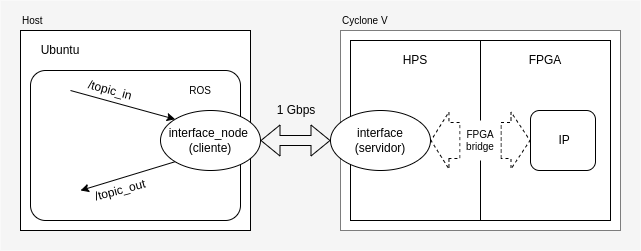
\includegraphics[scale=0.7]{imagens/arquitetura_geral.png}\\
		{\small \textbf{Fonte:} do autor}
    \end{center}\label{fig:arquitetura}
\end{figure}




\section{Biblioteca de comunicação - libinterfacesocket}

Para manter o padrão do desenvolvimentos dos códigos tanto do cliente quanto do servidor, foi desenvolvida uma classe que fornece os métodos para a abertura da comunicação, além de métodos para envio e recebimento das mensagens através da rede gigabit ethernet. Essa classe foi desenvolvida como um módulo à parte e compilada como uma biblioteca estática. sDesta forma, uma vez testados e validados seus  métodos de comunicação, tanto o código do cliente quanto o do servidor poderão fazer uso desta biblioteca, eliminando assim a necessidade de reescrever uma parte
do código. Outra vantagem nessa abordagem é que, ao manter o código desassociado tanto do servidor como do cliente, nos possibilita fazer alterações ou correções de erros, sem necessariamente realizar alterações nos códigos do servidor ou do cliente.

A programação da biblioteca foi realizada com base em \textit{sockets}. \textit{Sockets} são um caminho para conectar processos em uma rede de computadores. A conexão através de \textit{sockets} entre nós em uma rede independe do protocolo. Um nó da rede ouve uma determinada porta para um IP específico esperando por um pedido de conexão do segundo nó, assim a conexão entre dois processos é estabelecida. O servidor é o nó que aguarda o pedido ser enviado pelo cliente.

A programação de sockets em C++ possibilita um alto nível de otimização da comunicação entre os processos, principalmente por se tratar de um modelo cliente-servidor onde só existirá a comunicação entre o servidor e apenas um cliente. Após implementar a comunicação entre o servidor e o cliente, poderão ser testadas novas técnicas para otimizar o desempenho da rede possibilitando o aumento da taxa de transferência de dados entre o servidor e o cliente.

O código fonte da biblioteca pode ser encontrado no repositório no github~\cite{Pereira-Neto-Biblioteca}, que pode ser visto na figura~\ref{fig:gitlib}, onde podemos observar a estrutura de arquivos da blibioteca. Vale frizar que, a libinterfacesocket possui um makefile para realizar o processo de compilação de forma automática. Assim podemos de forma simplificada compilar e instalar a biblioteca tanto no sistema do host onde será executado o cliente, quanto no sistema do HPS embarcado no SoC, onde o servidor estará rodando. 

\begin{figure}[ht]
	\caption{Repositório libinterfacesocket}
	\begin{center}
		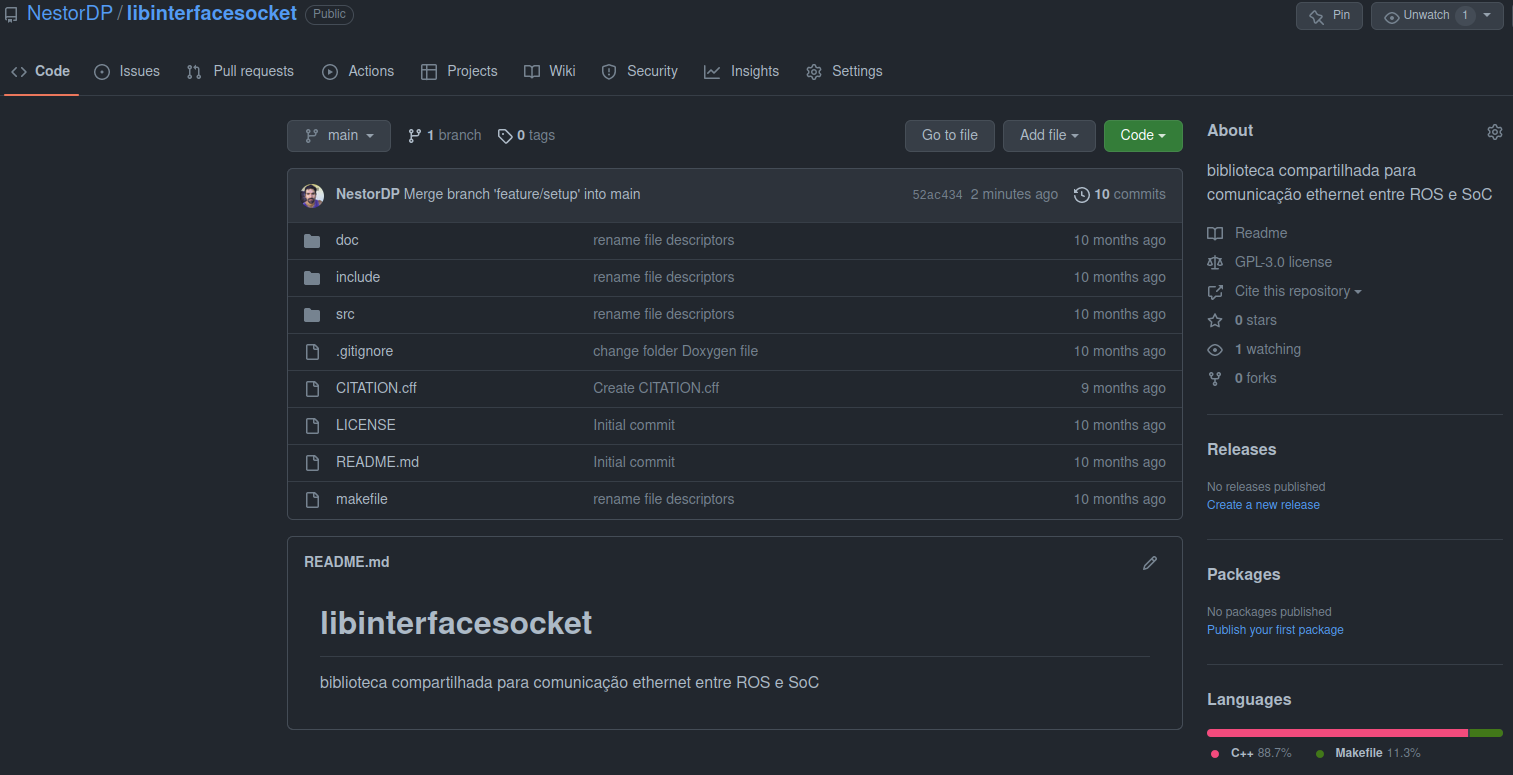
\includegraphics[scale=0.26]{imagens/git_libinterfacesocket.png}\\
		{\small \textbf{Fonte:} do autor}
    \end{center}\label{fig:gitlib}
\end{figure}
